%% LyX 2.2.1 created this file.  For more info, see http://www.lyx.org/.
%% Do not edit unless you really know what you are doing.
\documentclass[english,a4paper]{article}
\usepackage[T1]{fontenc}
\usepackage[latin9]{inputenc}
\usepackage{geometry}
\geometry{verbose,tmargin=1.5cm,bmargin=1.5cm,lmargin=2cm,rmargin=2cm}
\pagestyle{empty}
\usepackage{graphicx}

\makeatletter

%%%%%%%%%%%%%%%%%%%%%%%%%%%%%% LyX specific LaTeX commands.
%% Because html converters don't know tabularnewline
\providecommand{\tabularnewline}{\\}

\makeatother

\usepackage{babel}
\begin{document}

\title{2ID90 Spell Checker Assignment\\
\emph{template report} }

\author{Group XY: <name of author1>, <name of author2>}
\maketitle

\section{Introduction}

\emph{Give a short introduction on your program: state the objectives
and comment on how they are achieved. Further more, in the whole document,
please take care of the following:}
\begin{itemize}
\item \emph{Refer to any material you used to obtain your results}, e.g.
\cite{Ertel:2011:IAI:1971988}\emph{.}
\item \emph{Illustrate your material with appropriate figures which are
numbered and have a descriptive caption. Refer to the figure in the
text: see }Figure \ref{fig:DanJurafsky}\emph{.}
\begin{figure}[bh]
\begin{centering}
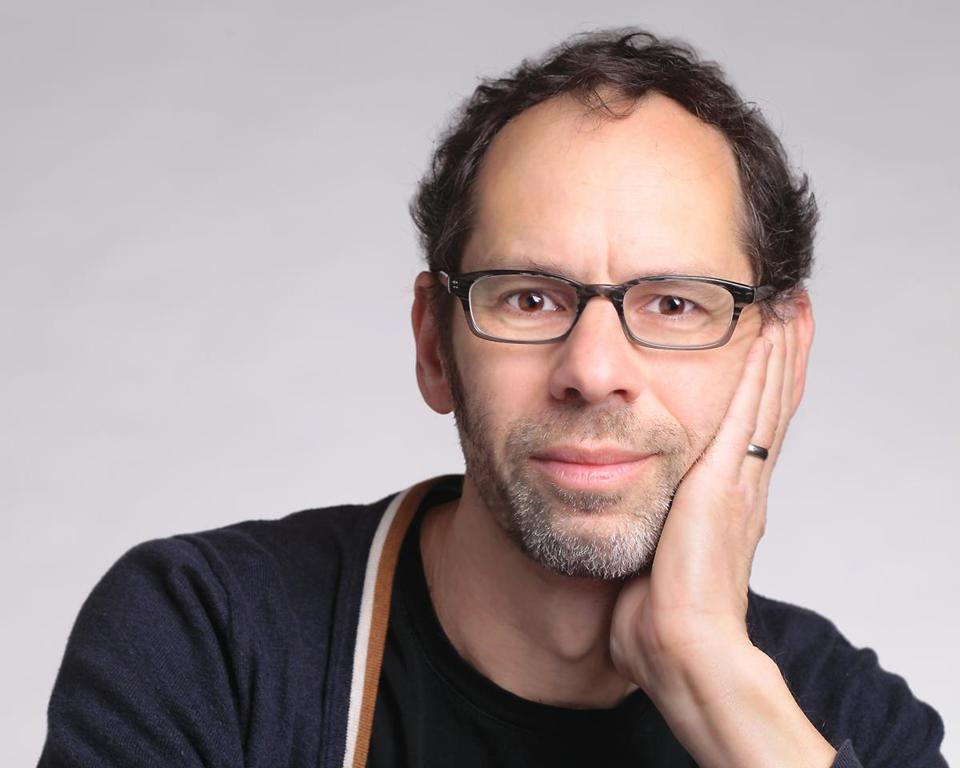
\includegraphics[scale=0.1]{DanJurafsky}
\par\end{centering}
\emph{\caption{\label{fig:DanJurafsky}The author of the book we used for background
information.}
}

\end{figure}
\item \emph{Use pseudo-code to explain your algorithms. Note that pseudo-code
is not the same as your actual java code. It should be an abstraction
of that code and should be presented with readability and clarity
in mind. Pseudo-code has to be accompanied with proper explanation
and argumentation.}
\item \emph{Use numbered mathematical formulas instead of lengthy explanations
in text. Additionally, discuss the principles behind the formula.}
\end{itemize}

\section{Overall approach }

\emph{Give a full discussion of how you have followed the general
set-up as given by the course material and how you have implemented
your spell checker.}

\section{Phrase generation and evaluation}

\emph{Give a full discussion of how you have implemented phrase generation
and have the best candidate sentence is selected. In particular, describe
what rule the confusion matrices and bigrams play a role in attaching
a value/probability to a candidate sentence. Also describe what type
of smoothing you use and how you have implemented it.}

\section{Results and evaluation}

\emph{Provide an overall assessment of your programs. What type of
errors is it good at to catch and repair, which type or errors are
missed or wrongly repaired. Explain what could be done, in principle,
to improve your program. Discuss how you have calibrated the relevant
parameters.}

\section{Advanced enhancements}

\emph{Several extensions and enhancements of the basic set-up of the
spell checker are possible. Describe explicitly what you have incorporated
from other sources than the course material to improve the performance
of your program and in what way the performance did improve indeed. }

\section{Conclusions and contributions}

\emph{A short logical summing up of the main reported results and
a statement on the contributions of each of the authors.}

\begin{tabular}{|c|c|c|c|}
\cline{2-4} 
\multicolumn{1}{c|}{} & \textbf{implementation} & \textbf{documentation} & \textbf{total \#hours}\tabularnewline
\hline 
Author 1 & 60\% & 30\% & 30\tabularnewline
\hline 
Author 2 & 40\% & 70\% & 25\tabularnewline
\hline 
\end{tabular}
\begin{itemize}
\item \emph{At least the given columns in the table need to be filled in,
add columns if needed.}
\item \emph{Add comments to clarify your table entries when necessary.}
\end{itemize}
\bibliographystyle{plain}
\bibliography{references}

\end{document}
